\subsection{Davide Rossi}
\subsubsection{Bank e Bankstate}
\emph{Problema}\newline
Come detto nell'architettura, \texttt{Bank} è l'entita che si occupa della parte di compravendita del gioco, gestendo i \texttt{Bank Account} dei giocatori 
e i \texttt{Title deed} associati alle caselle proprietà.
\texttt{Turnation Manager}, per arbitrare e gestire l'avanzamento del gioco, deve poter comunicare con la banca per richiedere o chiedere di modificare 
informazioni sulla situazioni finanziaria degli utenti. Ad esempio, quando il giocatore termina il turno bisogna
controllare se il suo \texttt{Bank Account} è in regola per la prosecuzione del gioco e se ha eseguito tutte le transazioni
obbligatorie nel suo turno, se il giocatore ha perso tutti i suoi contratti ritornano disponibili all'acquisto\dots\newline
\texttt{Turnation manager} deve quindi poter fare richieste alla banca per poter arbitrare la partita.\newline
\emph{Soluzione}\newline
Inizialmente era stato delegato al GameController il compito di mediatore fra i due componenti. 
Tuttavia questo poneva molta responsabilità sul controller aumentandone la complessità e rendendolo più fragile, esponendo l'applicazione a bug vari
che si potrebbero originare qualora questo non utilizzasse i componenti in maniera corretta. 
In più, il controller doveva reperire dalla banca e poi passare a \texttt{Turnation Manager} le informazioni necessarie per gestire l'avvicendarsi 
dei turni di gioco oppure utilizzare queste informazioni per delle operazioni di logica di dominio che non sarebbero di sua responsabilità.\newline
\texttt{Turnation Manager} non era quindi progettato per operare in maniera autonoma. \newline
Rifacendoci all'analisi, si è pensato di implementare una qualche sorta di comunicazione fra \texttt{Turnation Manager} e \texttt{Bank}. Utilizzando il pattern "Adapter" 
\texttt{BankStateAdapter} (Adapter) fa uso dei metodi interni di \texttt{BankImpl} (Adaptee) per garantire che questa classe aderisca 
a un'interfaccia scritta apposta per \texttt{Turnation Manager}: \texttt{BankState}.
In questo modo \texttt{BankImpl} aderisce a due interfacce
specifiche per i suoi due utilizzatori: il controller usa \texttt{Bank} come unico punto d'accesso per l'esecuzione di transazioni, e grazie a \texttt{BankStateAdapter} \texttt{Turnation manager} può fare uso di 
un oggetto \texttt{BankState} per controllare la situazione bancaria dei giocatori e orchestrare il ciclo di vita della partita senza dipendere dal controller.
Infatti, parte delle operazioni di logica del dominio svolte dal controller precedentemente sono state rilocate in \texttt{Turnation Manager} come di diritto, in favore di un migliore incapsulamento e una 
maggiore facilità di utilizzo di questo componente dall'esterno. 
Allo stesso tempo il fatto che ogni client lavori con un'interfaccia scritta su misura per se limita le operazioni che ognuno può eseguire garantendo maggiore sicurezza e separazione degli interessi.\newline
\begin{figure}[H]
    \centering
    \makebox[1.0\textwidth]{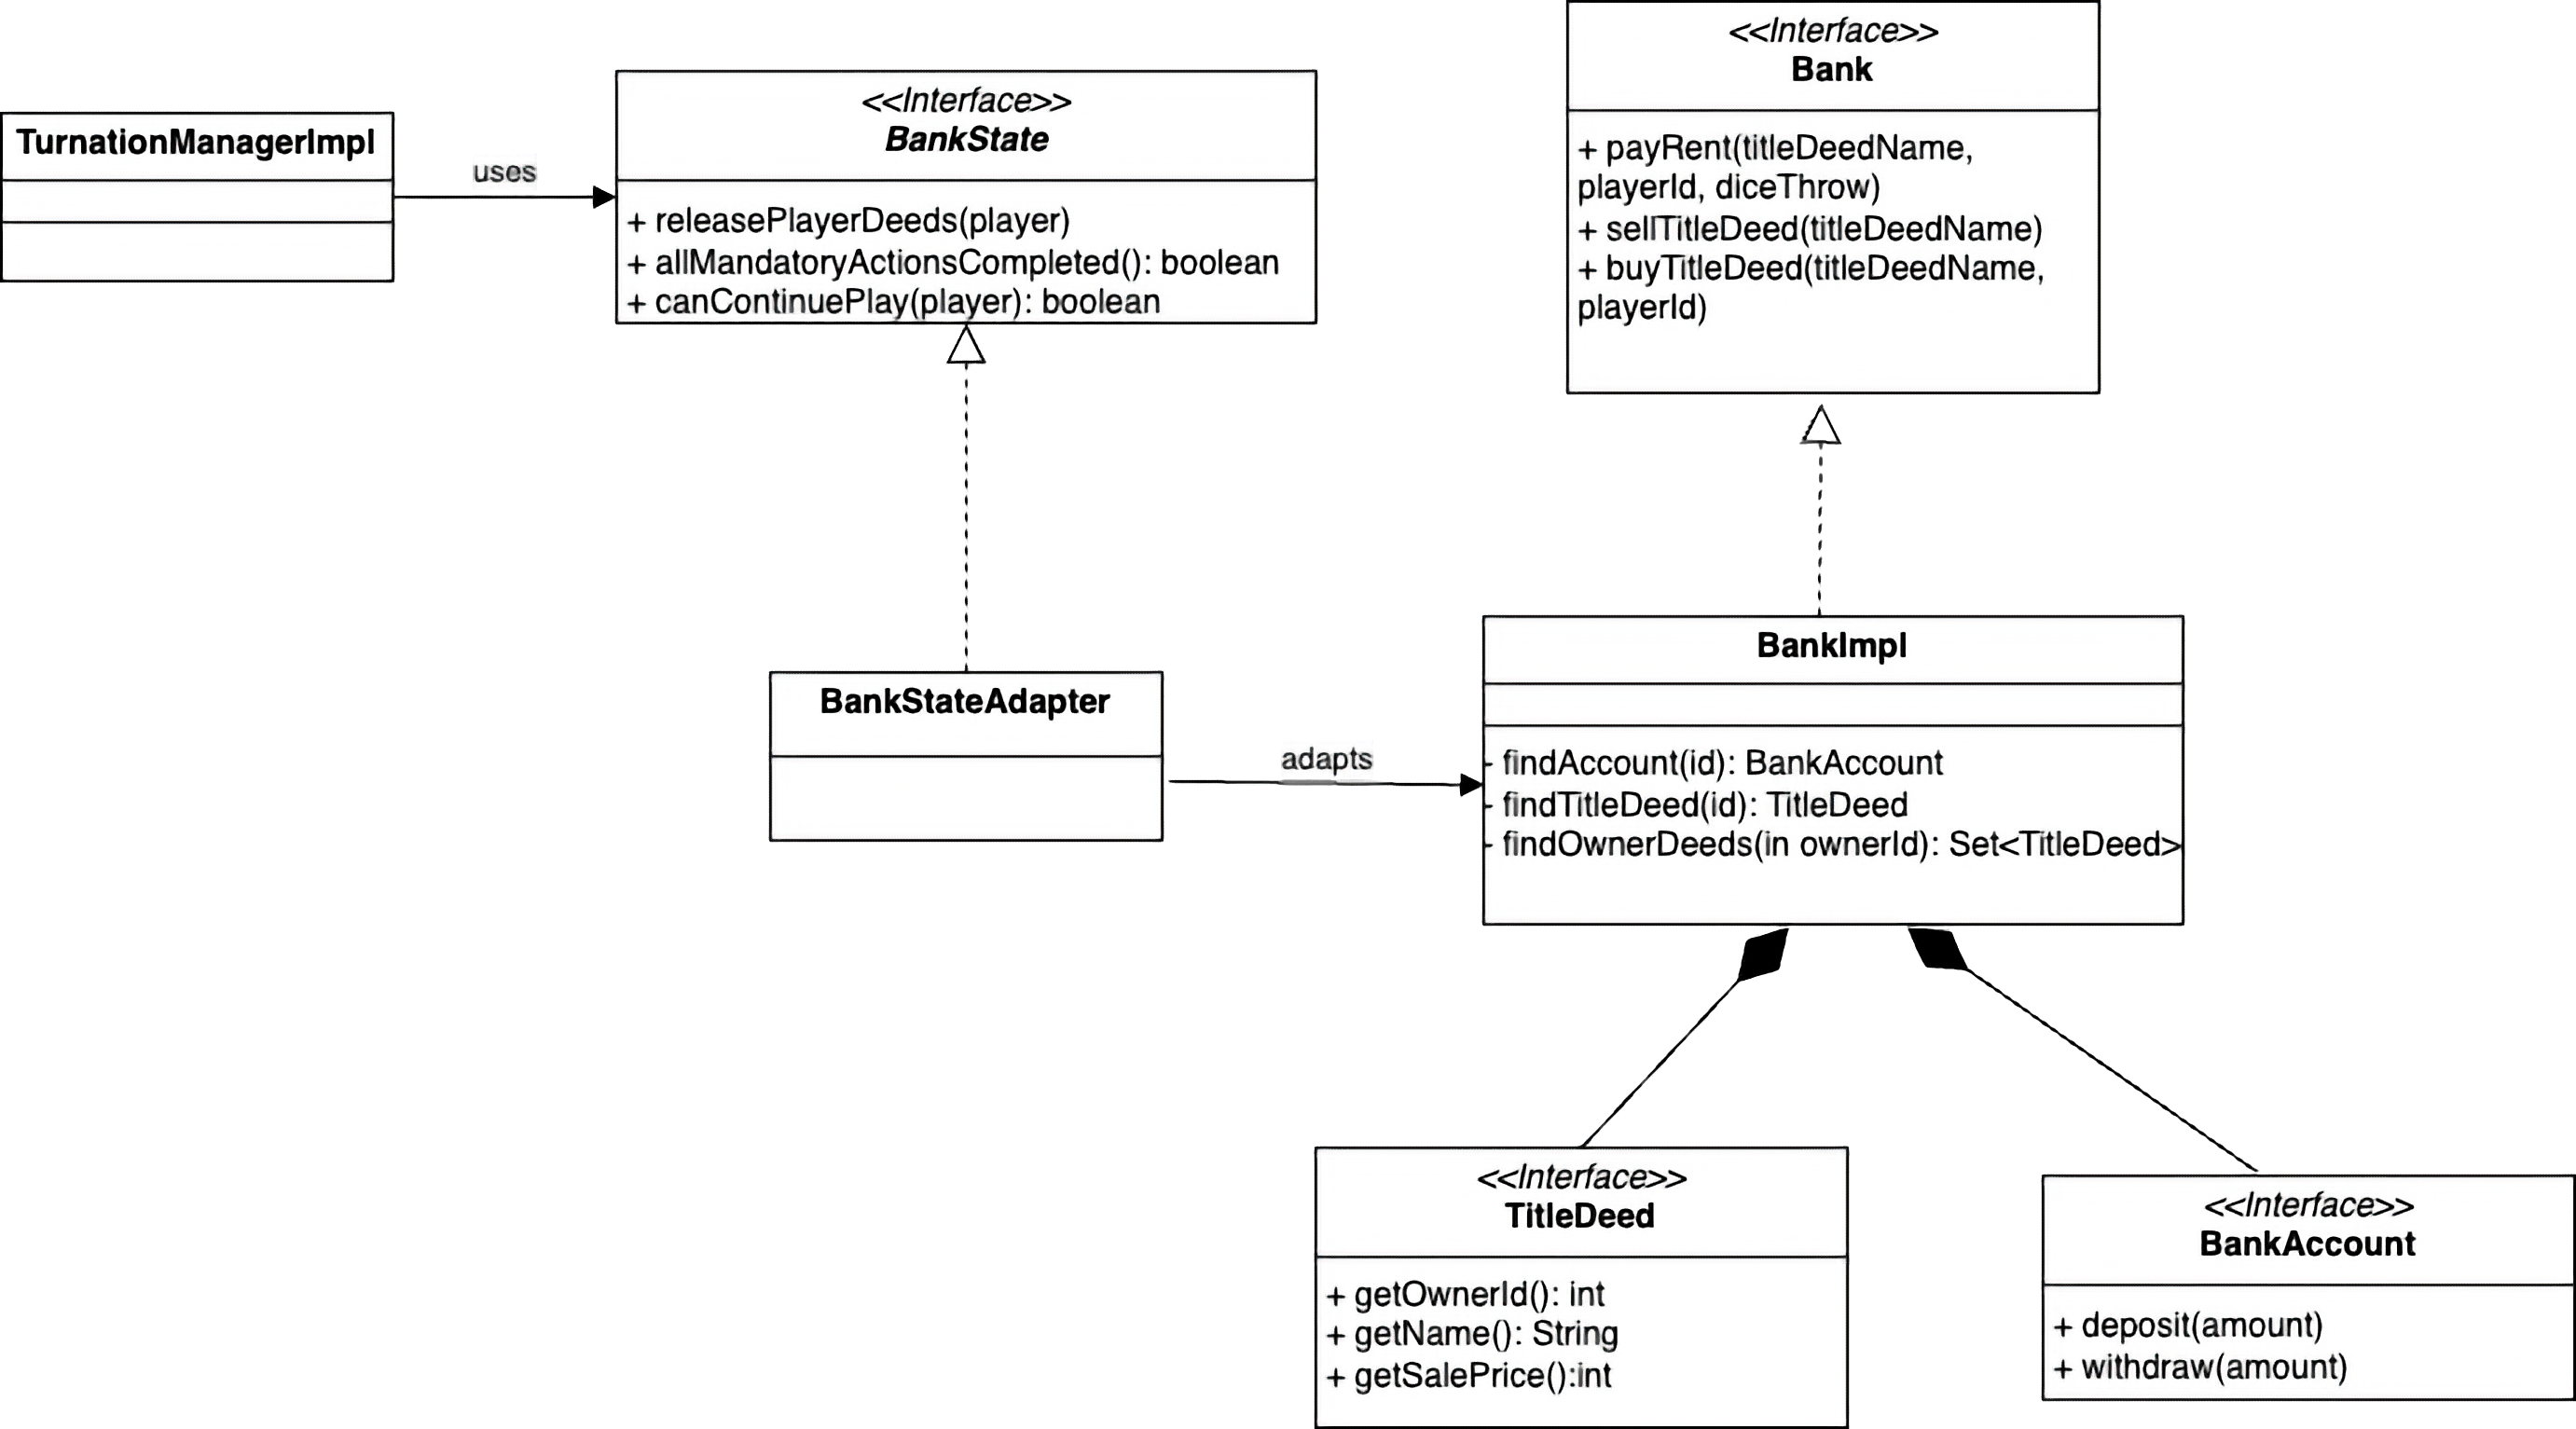
\includegraphics[width=1.3\textwidth]{img/rossi/bankStateAdapter.png}}	
    \caption{Schema UML del pattern Adapter. L'Adapter BankStateAdapter adatta l'oggetto BankImpl all'interfaccia BankState. TurnationManagerImpl utilizza
    un oggetto BankState per pilotare il gioco. Il controller, qui non riportato per chiarezza, ha un riferimento a un oggetto Bank}
	\label{img:bankstate}
\end{figure}
\subsubsection{Modellazione dei contratti di proprietà}
\emph{Problema}\newline
Rappresentare in un'unico oggetto tutte le informazioni di un contratto di proprietà. In particolare le opzioni di affitto, l'ipoteca e i costi di costruzione, 
in maniera flessibile e espandibile\newline
\emph{Soluzione}\newline
Si è deciso di adottare il pattern \say{decorator} per rendere il supporto alle case e alberghi una funzionalità componibile in
maniera flessibile, in modo da lasciare agli utilizzatori della classe la scelta di quale implementazione usare permettendo eventualmente di introdurre
più modalità di gioco. Lo stesso concetto si può
estendere introducendo nuovi decoratori per nuove versioni di \texttt{Title deed} per introdurre nuove funzionalità sui contratti.\newline
\texttt{TitleDeedDecorator} (decoratore) è una classe abstract che incapsula un oggetto di tipo \texttt{Title deed} (decorated) e aderisce alla suddetta interfaccia. 
\texttt{TitleDeedWithHouses} estende questa classe e modifica i metodi riportati nello schema, aggiungendo il supporto per il calcolo del costo di costruzione delle case e dell'albergo, 
e per il calcolo dell'affitto (\texttt{getRent}) considerando anche i miglioramenti
(case e albergo) piazzati sulla proprietà.\newline
Analizzando le regole del gioco si è notato che i metodi \say{costo} (\texttt{getHousePrice, getHotelPrice, getMortagePrice}\dots) 
calcolano i prezzi basandosi sul prezzo di vendita (\texttt{getSalePrice}) del contratto. Per implementare questi metodi in maniera flessibile 
si è deciso di usare il pattern \say{strategy}:
i vari metodi \say{costo} fanno uso di funzioni matematiche che prendono come input il prezzo di vendita. Queste funzioni, o algoritmi, 
vengono richieste al momento della creazione dell'oggetto lasciando all'utilizzatore la libertà di definirli e personalizzare il contratto.\newline
Ogni implementazione del contratto richiede gli algoritmi necessari per il suo specifico funzionamento\newline
\begin{figure}[H]
    \centering
    \makebox[0.5\textwidth]{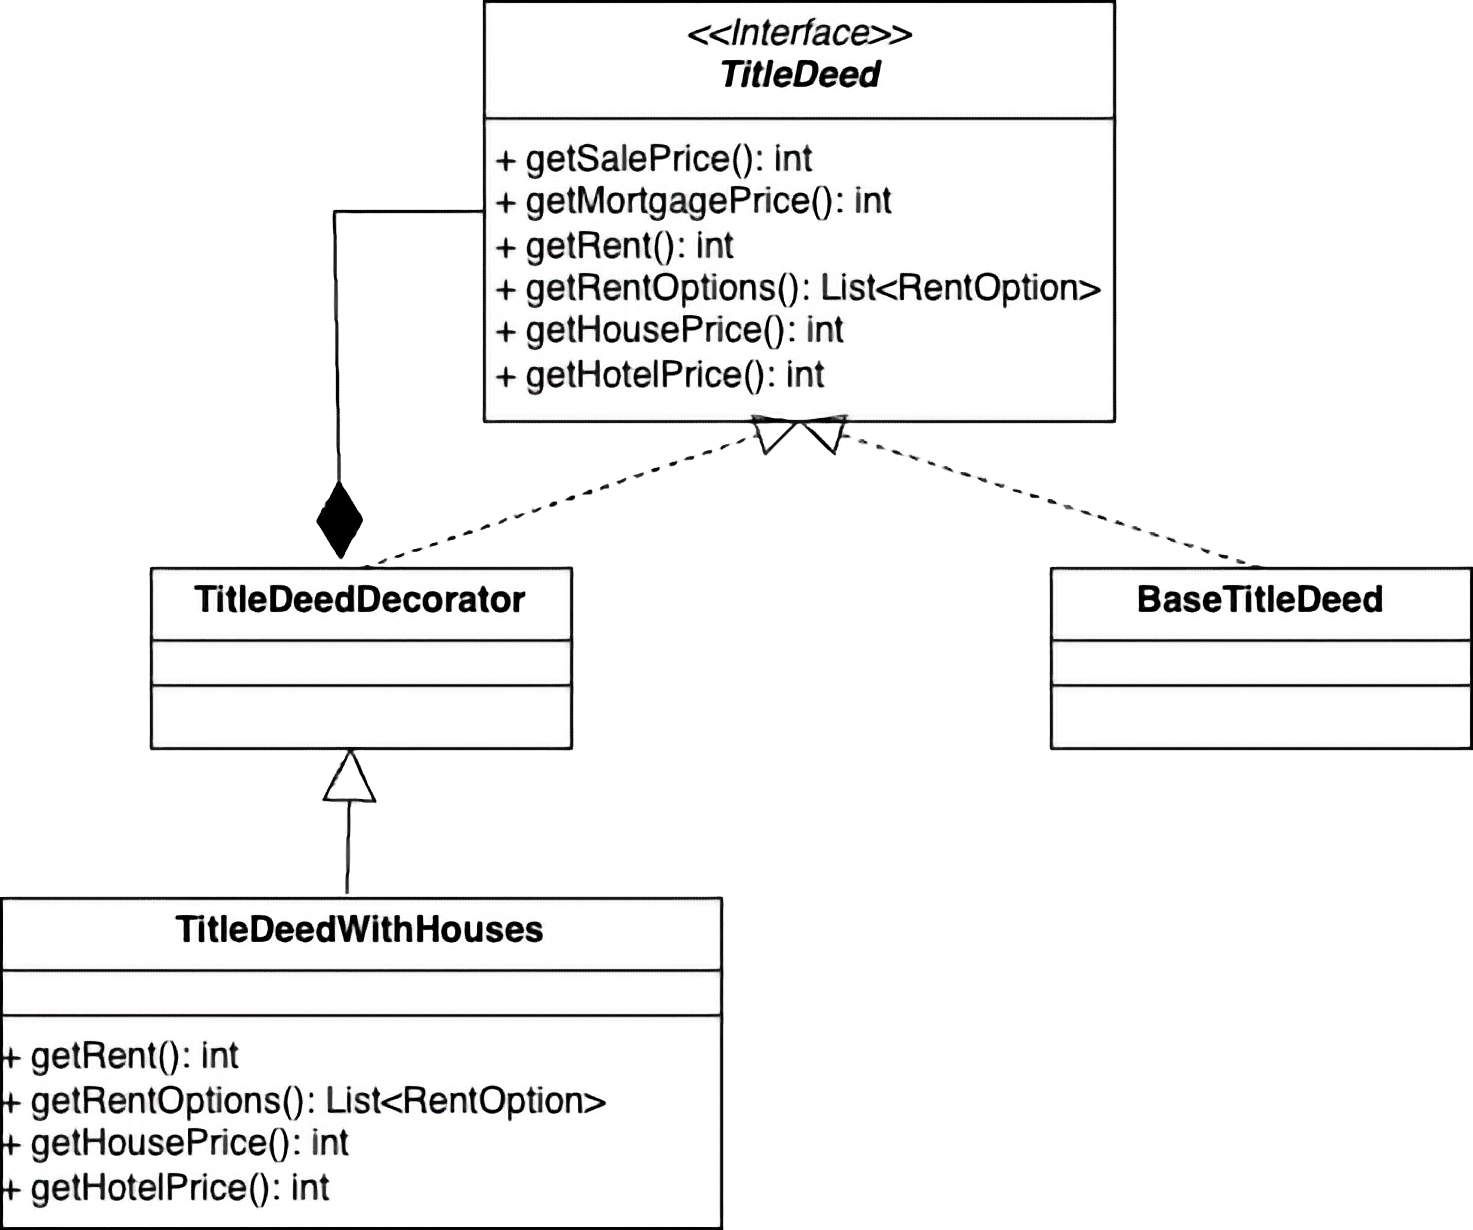
\includegraphics[width=0.8\textwidth]{img/rossi/titleDeed.png}}	
    \caption{Architettura dei contratti di proprietà. BaseTitleDeed è l'implementazione standard dell'interfaccia, è una tipologia di 
    contratto che non ha il supporto per la compravendita delle case. TitleDeedWithHouses reimplementa solo alcuni dei metodi dell' interfaccia
    mentre i rimanenti chiamano il metodo corrispondente sull'oggetto decorated}
	\label{img:TitleDeed}
\end{figure}
\subsubsection{Opzioni di affitto e fabbrica delle opzioni}
\emph{Problema}\newline
Rappresentare le varie opzioni d'affitto per ogni contratto di proprietà. Ogni
opzione di affitto ha un suo prezzo e dei criteri di applicabilità. 
Quando si richiede l’affitto per un contratto di proprietà, generalmente perchè
la pedina di un giocatore è capitata su una proprietà non sua ed esso deve pagare,
si consulta il contratto e si valuta quali opzioni di affitto sono applicabili.
Poi ne viene scelta una (solitamente la più costosa)
e il suo prezzo sarà il prezzo concordato per l'affitto.\newline
\emph{Soluzione}\newline
È stata creata un' interfaccia \texttt{Rent Option} 
con dei metodi per richiedere il prezzo e verificare se la suddetta Rent Option può essere applicata o meno, 
ogni \texttt{TitleDeed} ha un elenco di \texttt{RentOption}.\newline
Per facilitarne la creazione è stata realizzata una 
\texttt{RentOptionFactory} implementando il pattern \say{Abstract factory}. 
La factory permette di creare le principali tipologie di opzioni di affitto presenti nel gioco 
offrendo un certo grado di personalizzazione.\newline
\begin{figure}[H]
    \centering
    \makebox[1.0\textwidth]{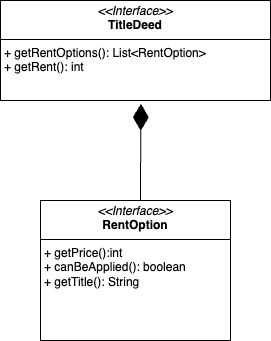
\includegraphics[width=0.4\textwidth]{img/rossi/rent_option.png}}	
    \caption{Rappresentazione dell'architettura di Title Deed e RentOption}
	\label{img:RentOption}
\end{figure}
\begin{figure}[H]
    \centering
    \makebox[1.0\textwidth]{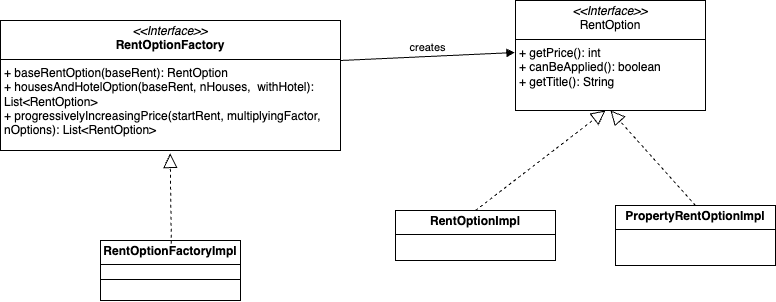
\includegraphics[width=1.1\textwidth]{img/rossi/rent_option_factory.png}}	
    \caption{Schema UML della factory di RentOption, la factory viene utilizzata dalla parte del sistema che si occupa di creare i contratti. 
    RentOptionFactoryImpl è l'unica implementazione dell'interfaccia RentOptionFactory}
	\label{img:RentOptionFactory}
\end{figure}
\subsubsection{Azioni sulle proprietà}
\emph{Problema}\newline
Quando il giocatore finisce su una casella \say{Property}
esso può/deve svolgere determinate azioni nel suo turno. 
La banca, controllando il \texttt{TitleDeed} corrispondente alla casella Property,  
deve notificare all' utente quali azioni può/ deve compiere\newline
\emph{Soluzione}\newline
Si è deciso di applicare il pattern \say{command}. 
Chiamando \texttt{getActionsForTitleDeed} \texttt{Bank} 
restituisce degli oggetti di tipo \texttt{PropertyAction}, 
che sono l'effettivo comando ed incapsulano il codice dell' azione eseguibile.
Il controller poi chiede alla view di mostrare le azioni all' utente, 
che potrà selezionare quale eseguire chiamando \texttt{executeAction} sul controller.\newline 
In questo modo è estremamente facile estendere il gioco 
con nuove funzionalità creando nuove \texttt{PropertyAction} senza 
modificare il controller.\newline
Per rendere più facile la creazione sul momento delle azioni e 
migliorare la riusabilità è stata creata un’ \say{abstract factory} 
con le azioni principali tipiche del gioco.
\begin{figure}[H]
    \centering
    \makebox[1.0\textwidth]{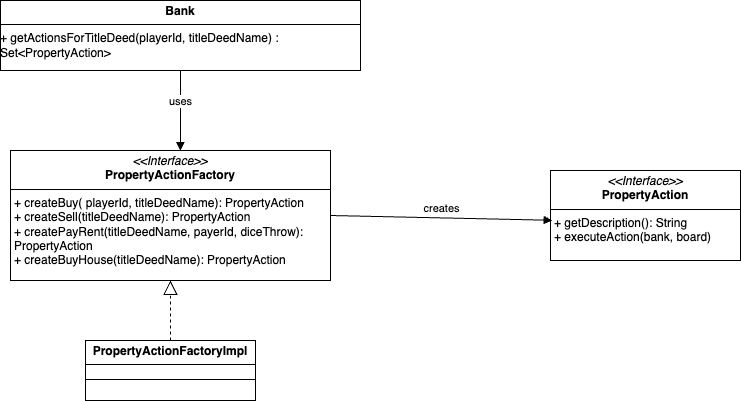
\includegraphics[width=1.0\textwidth]{img/rossi/property_action.png}}	
    \caption{PropertyActionFactory è la factory che si occupa di creare le PropertyAction. Bank controlla quali azioni sono concesse all'utente selezionato
    per il determinato contratto selezionato e adopera la factory per creare i comandi}
	\label{img:PropertyAction}
\end{figure}